In this approach our task is to reach the target set avoiding obstacles. Our Simulations are divided in 2 main cases: 
\begin{itemize}
    \item The first one takes place in a static environment, where we have fixed obstacles and a fixed target set 
    \item The second one takes place in a dynamic environment with moving obstacles and a moving target set.
\end{itemize}
The second case contains 3 sub-cases:  
\begin{itemize}
    \item The Robot is near the target set
    \item The Robot is distant from the target set
    \item The Robot is outside the $RAS$ (Reach-Avoid Set)
\end{itemize}
In addiction there are other simulations of all these cases with 2 different types of disturbances: 
\begin{itemize}
    \item Optimal Disturbance
    \item Random Disturbance
\end{itemize}
So we will see how the robot performs better actions against a random disturbance
\subsection{Static Case}
    As mentioned before in this case the robot has to reach a fixed target set wich is among some rectangular fixed obstacles. The simulation develops in a time of 10 seconds.
    We can start seeing the $RAS$ in different instants of time to see its expansion during the regression.
    
    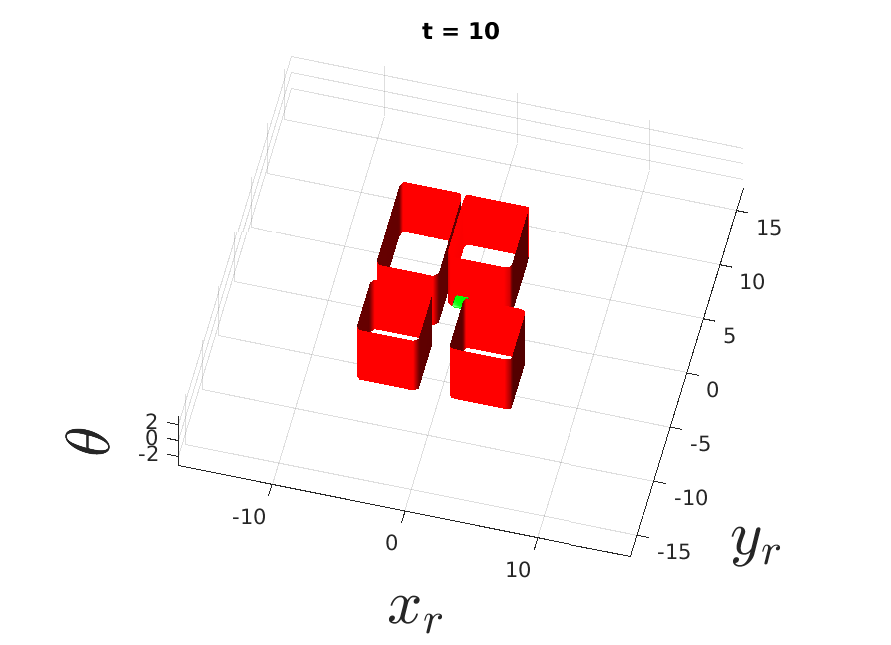
\includegraphics[scale=0.6]{figures/staticRAS1.png}
    
    The 2 horizontal axis represent the X-axis and the Y-xis, while the third one represents the angle Theta: the angle that the X-axis in the robot framework forms with the X-axis of the World Reference Framework.  
    Here we can notice a small green area which represents the target set and 4 red
    rectangles representing the obstacles. Since this representation takes place in the configuration space the obstacles are bigger than their real dimension and the target set seems smaller.
    It is evident from the target set that the robot is not allowed to reach the target set in any possible orientation, but only in a small range around the 0 $rad$ so we expect to see some maneuvers to adjust the orientation.  
    Then we can see the expansion of the $RAS$ to its final limits.
    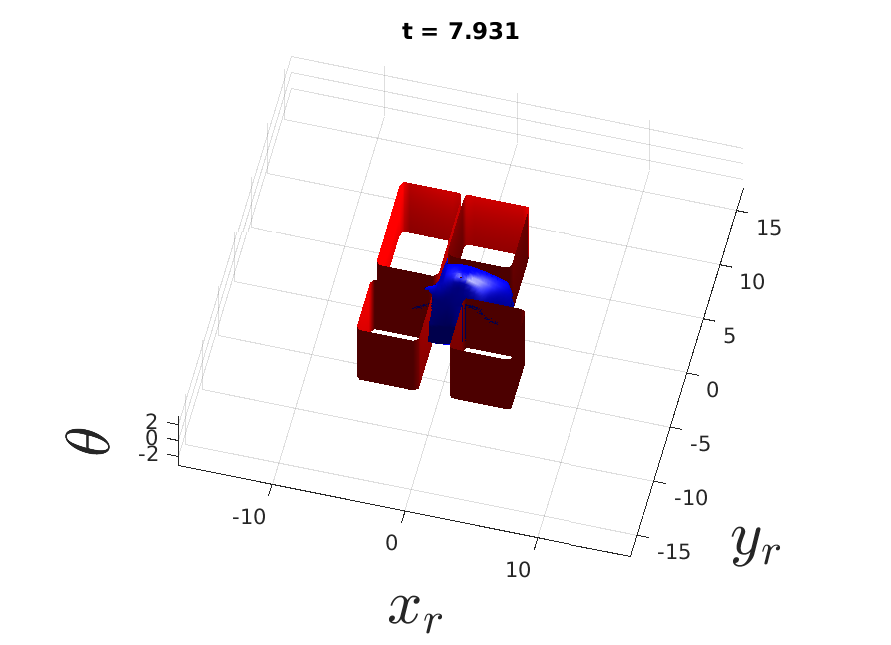
\includegraphics[scale=0.6]{figures/staticRAS2.png}
    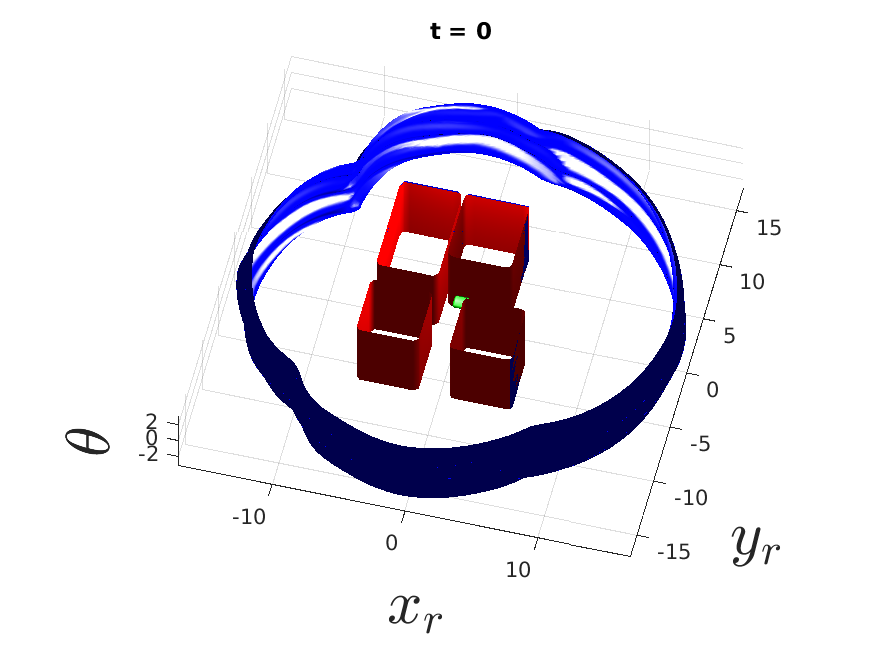
\includegraphics[scale=0.6]{figures/staticRAS3.png}
    The blue area represents the border of the Reach-Avoid Set. So from any initial configuration $(x_{i},y_{i},\theta{i})$ inside the blue border our robot is expected to reach the target set in the time limit of 10 seconds. 
    Now that the $RAS$ is defined we can see how the robot reaches the target set avoiding obstacles and playing against an optimal disturbance.
    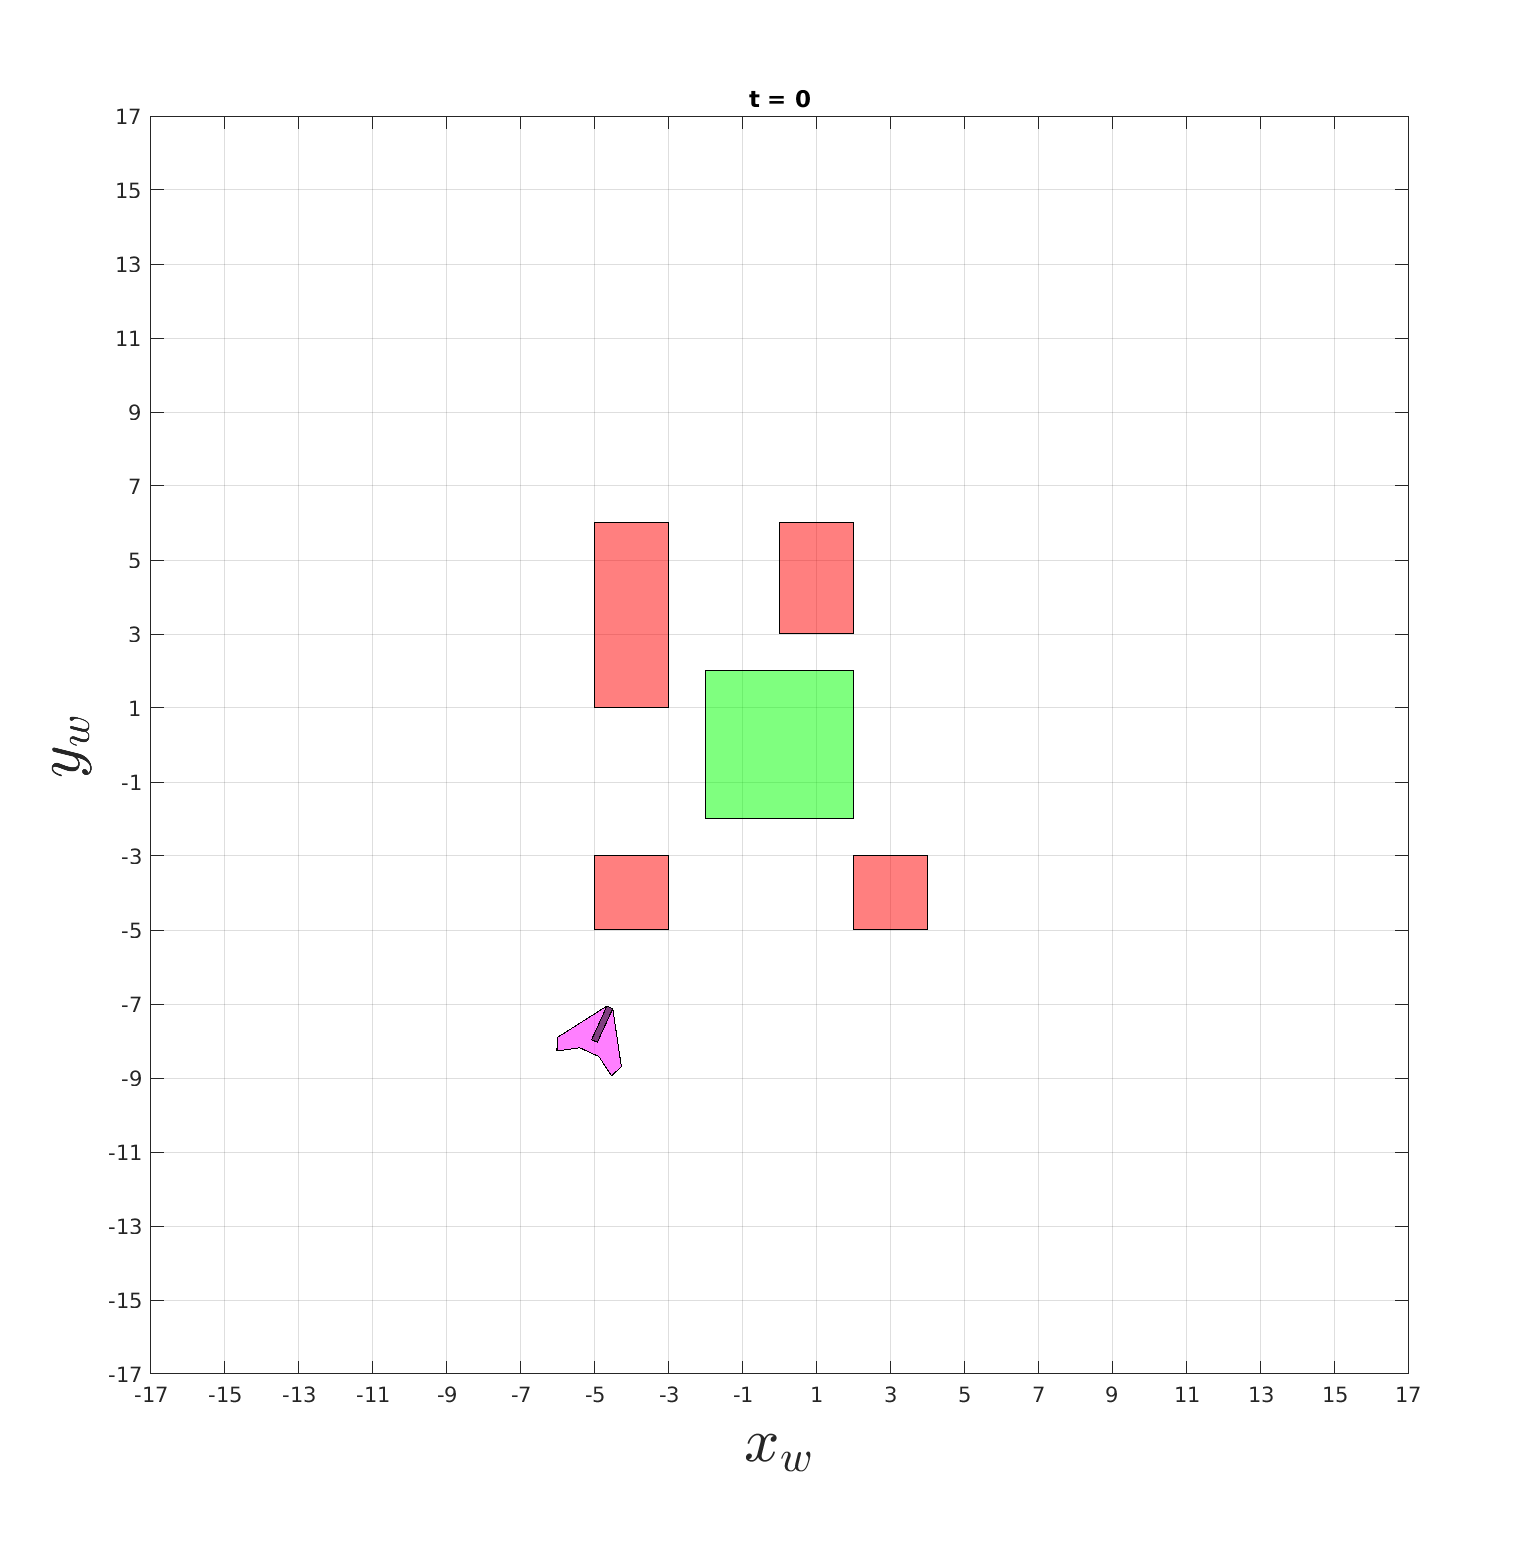
\includegraphics[scale=0.3]{figures/staticTRAJ1.png}
    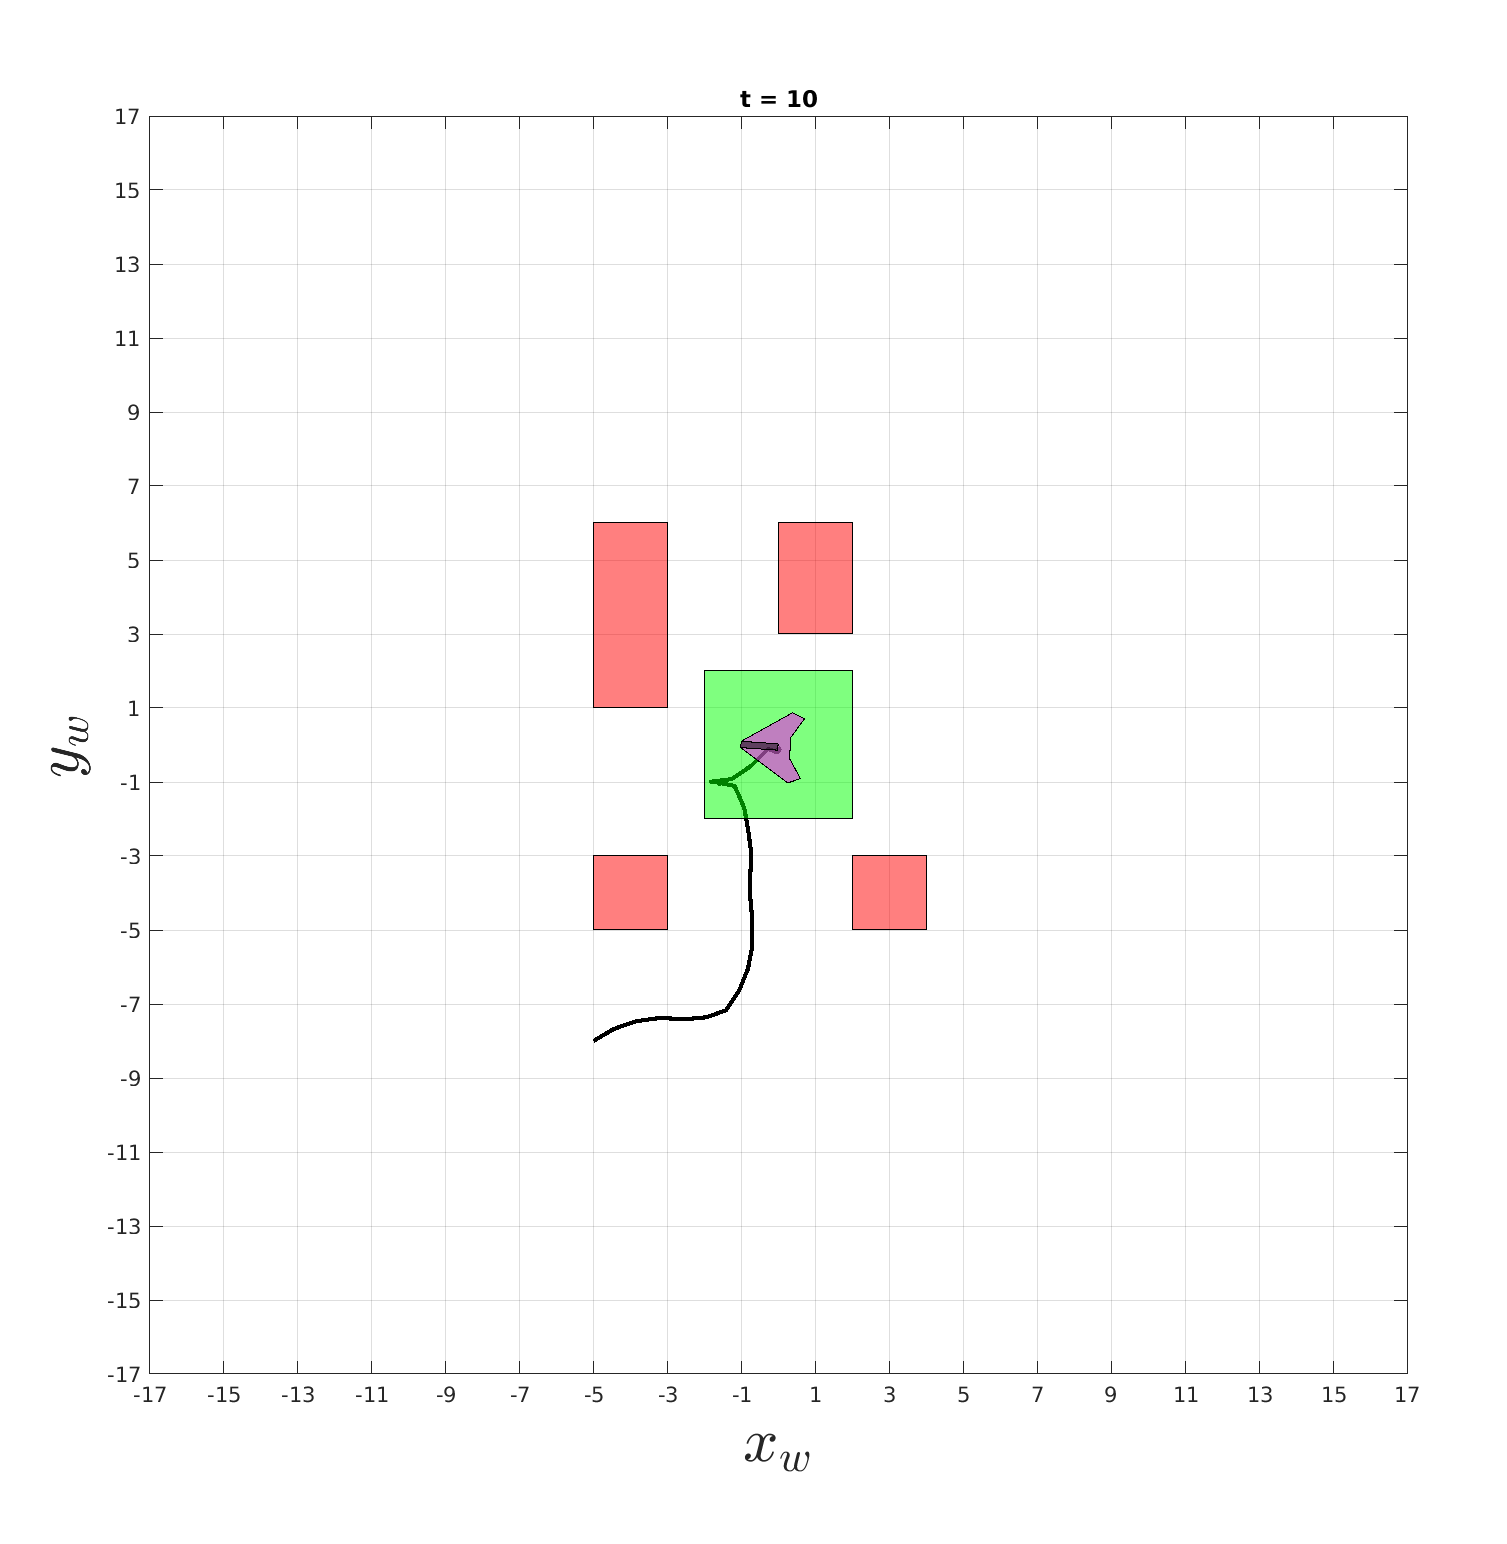
\includegraphics[scale=0.33]{figures/staticTRAJ2.png}
    So since the robot's initial position is in the limits of the $RAS$ we can see that it reaches, after the needed time, the target set in the desired angulation, avoiding the obstacles in its path. To conclude this case we can see the control inputs values playing against the optimal disturbance.
    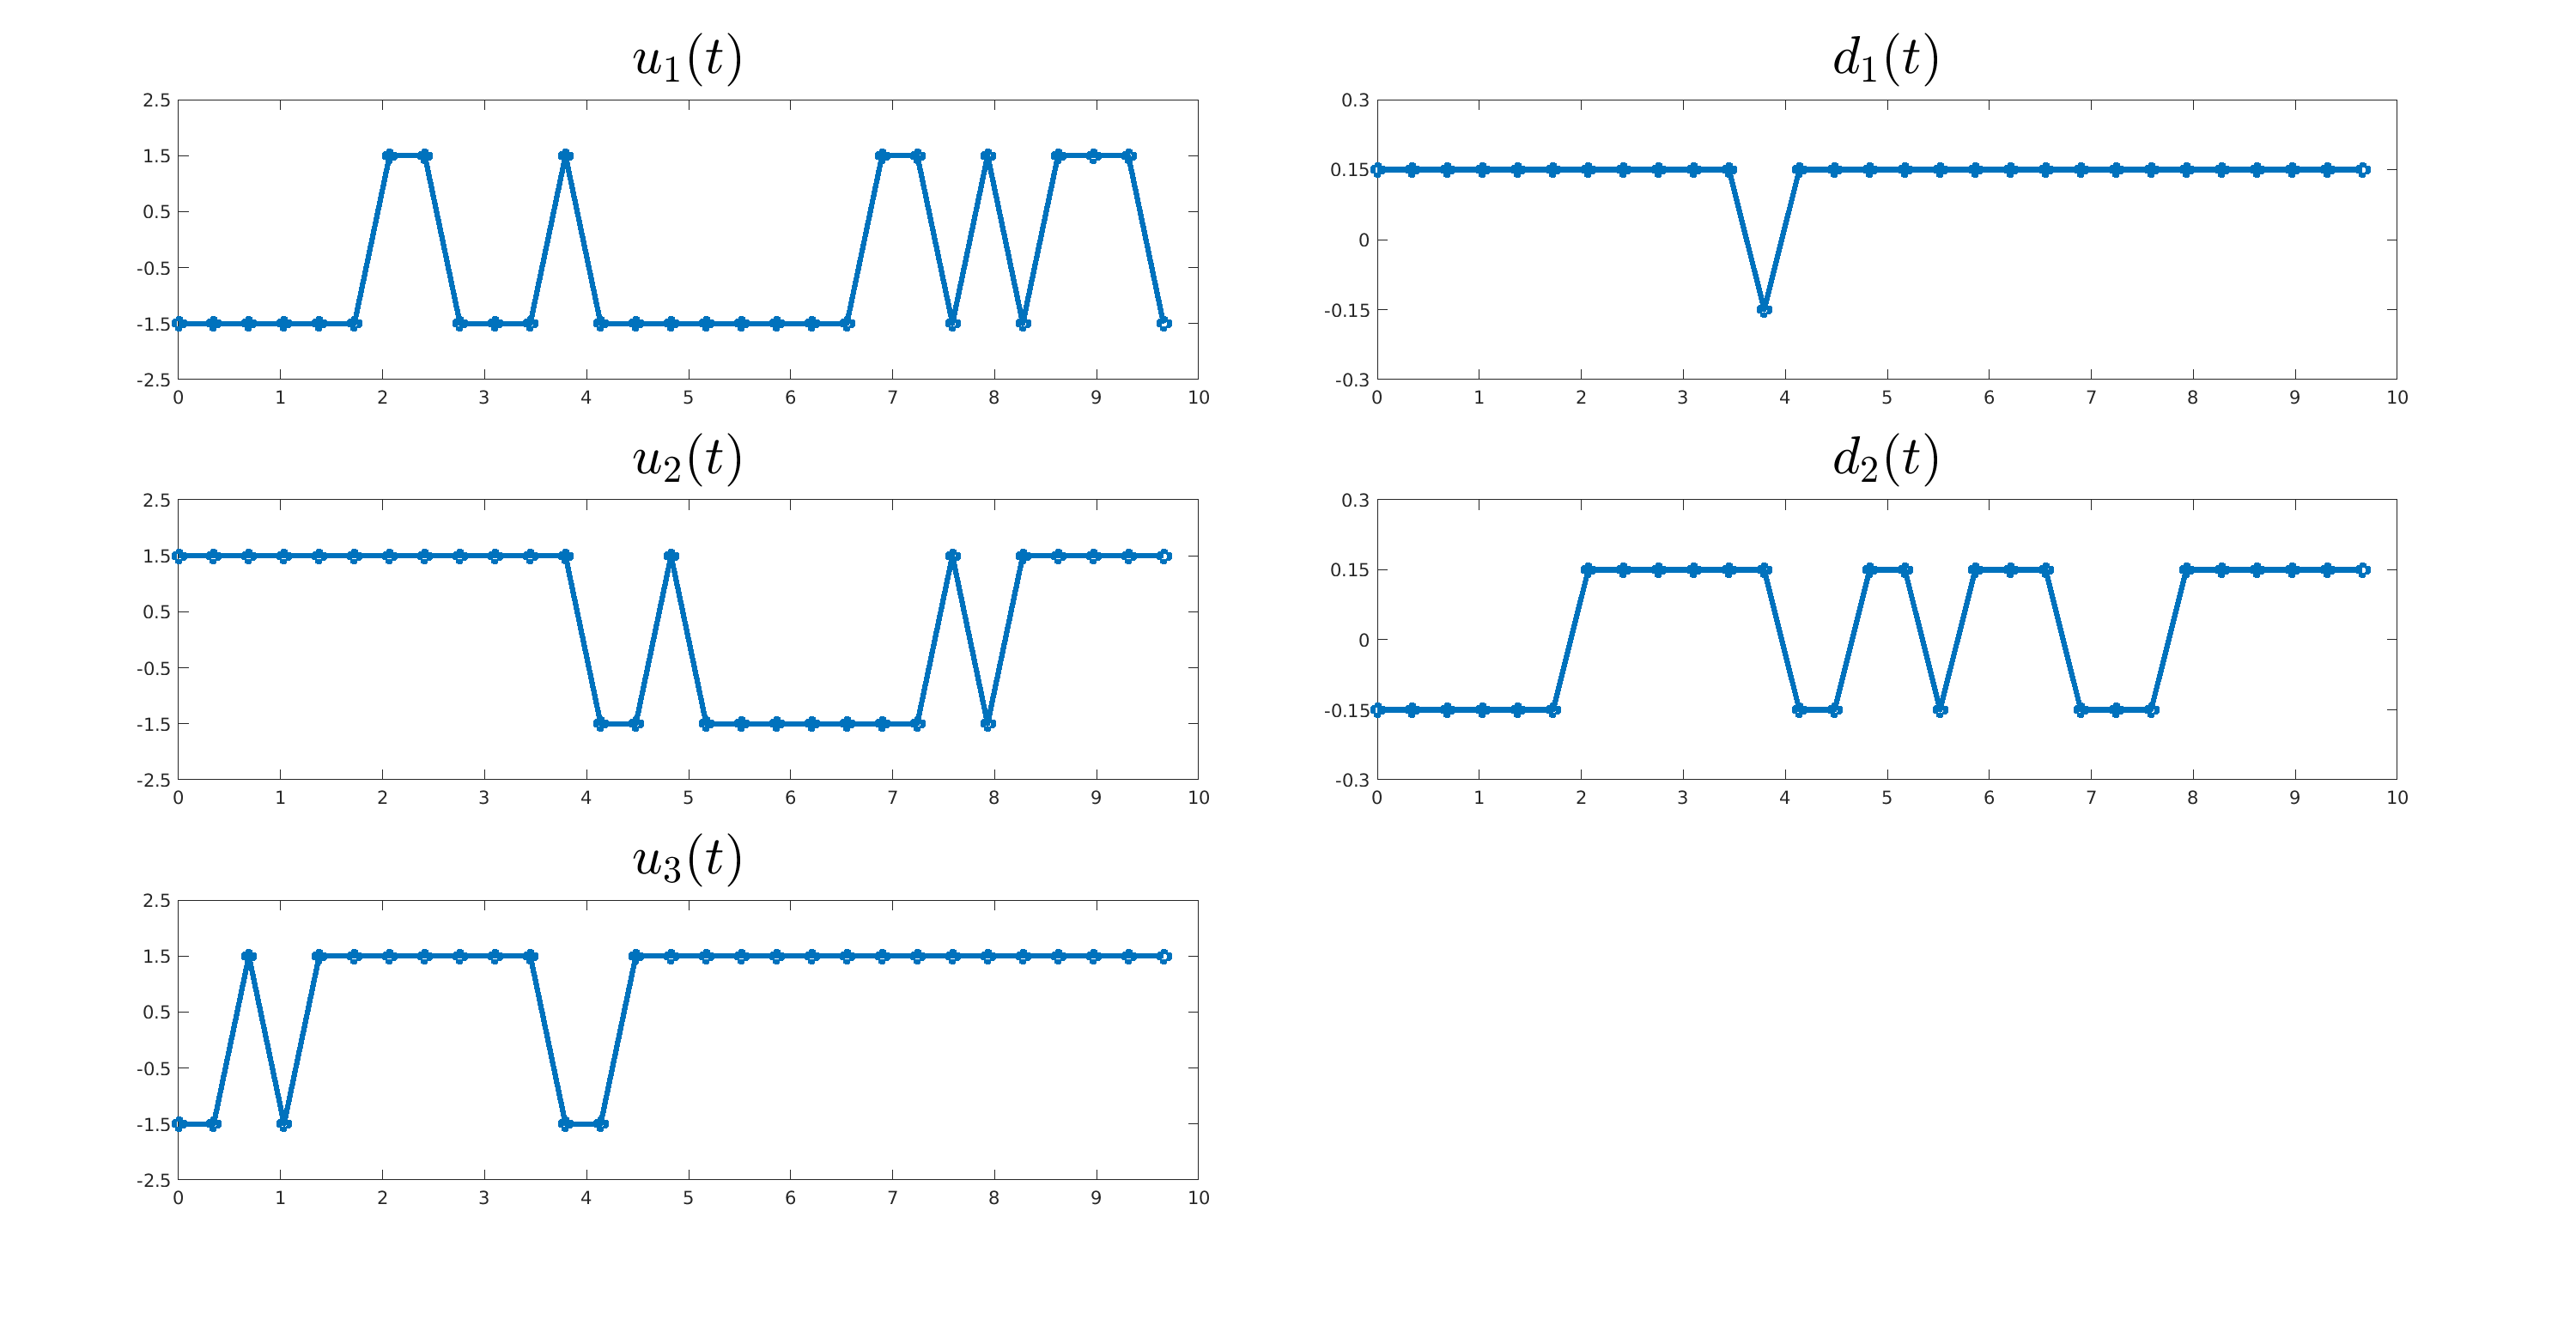
\includegraphics[scale=0.18]{figures/staticCONTROL1.png}
\subsection{Dynamic Case}
    Now we will see some more complex cases where the objects are not fixed, but they move in the environment. Here we simulated a moving platform which represent a recharging station for the robot. So the robot has to access the platform while this platform is moving downward along the Y-axis. The platform is not accessible from everywhere, but only from the right side, while the other sides are surrounded by obstacles. As mentioned before, we simulated three different cases for the Dynamic experiments. We are going to see the $RAS$ developing over time in a particular direction since the target set (always represented by a green area) is moving. The next figure represents the $RAS$ at time 10 seconds (so still not expanded). As mentioned before this represents a platform that can be entered just by one side and surrounded by obstacles. Since we are always in the configuration space we can not see the small target set which is surrounded by the red obstacles which seem bigger in the C-space.
    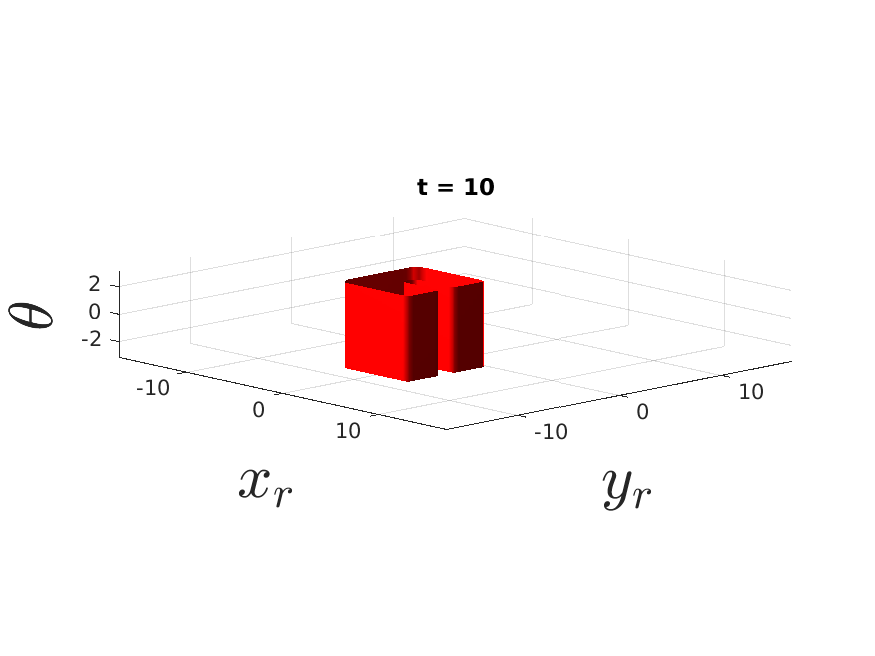
\includegraphics[scale=0.6]{figures/dynamicRAS1.png}
    At the end of the expansion of the $RAS$, so at time 0 seconds, we can see below the limits of the Set.
    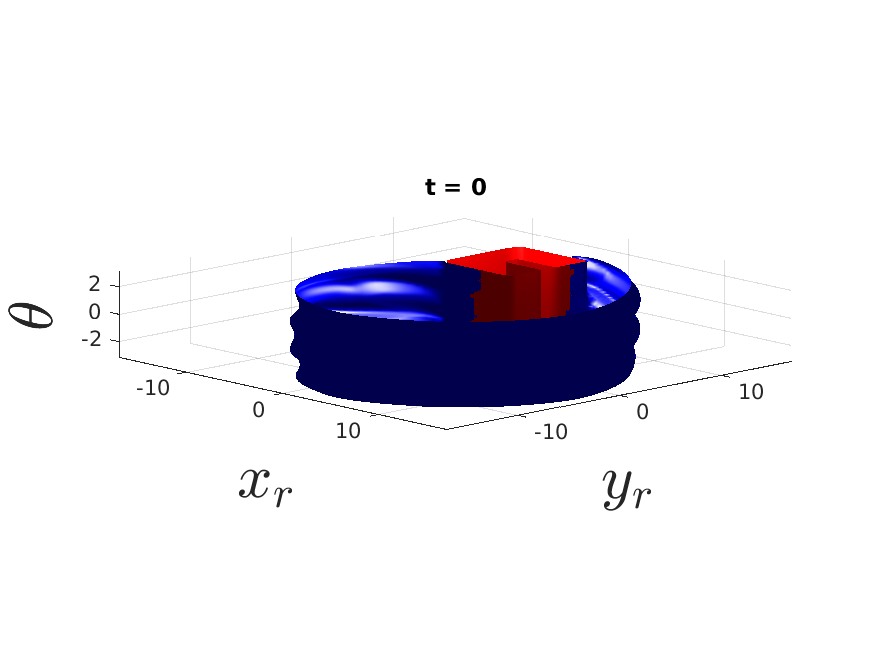
\includegraphics[scale=0.6]{figures/dynamicRAS2.png}
    We will see in each specific case a 2D representation of the $RAS$ to better understand the position of the target set and the different initial positions of the robot.
    \subsubsection{Case 1}
    In this first case the initial position of the robot is relatively near the target set and inside the $RAS$ at time 0 seconds, so we know from the theory that exists a trajectory which can lead the robot inside the target set in the maximum given time (10 seconds).
    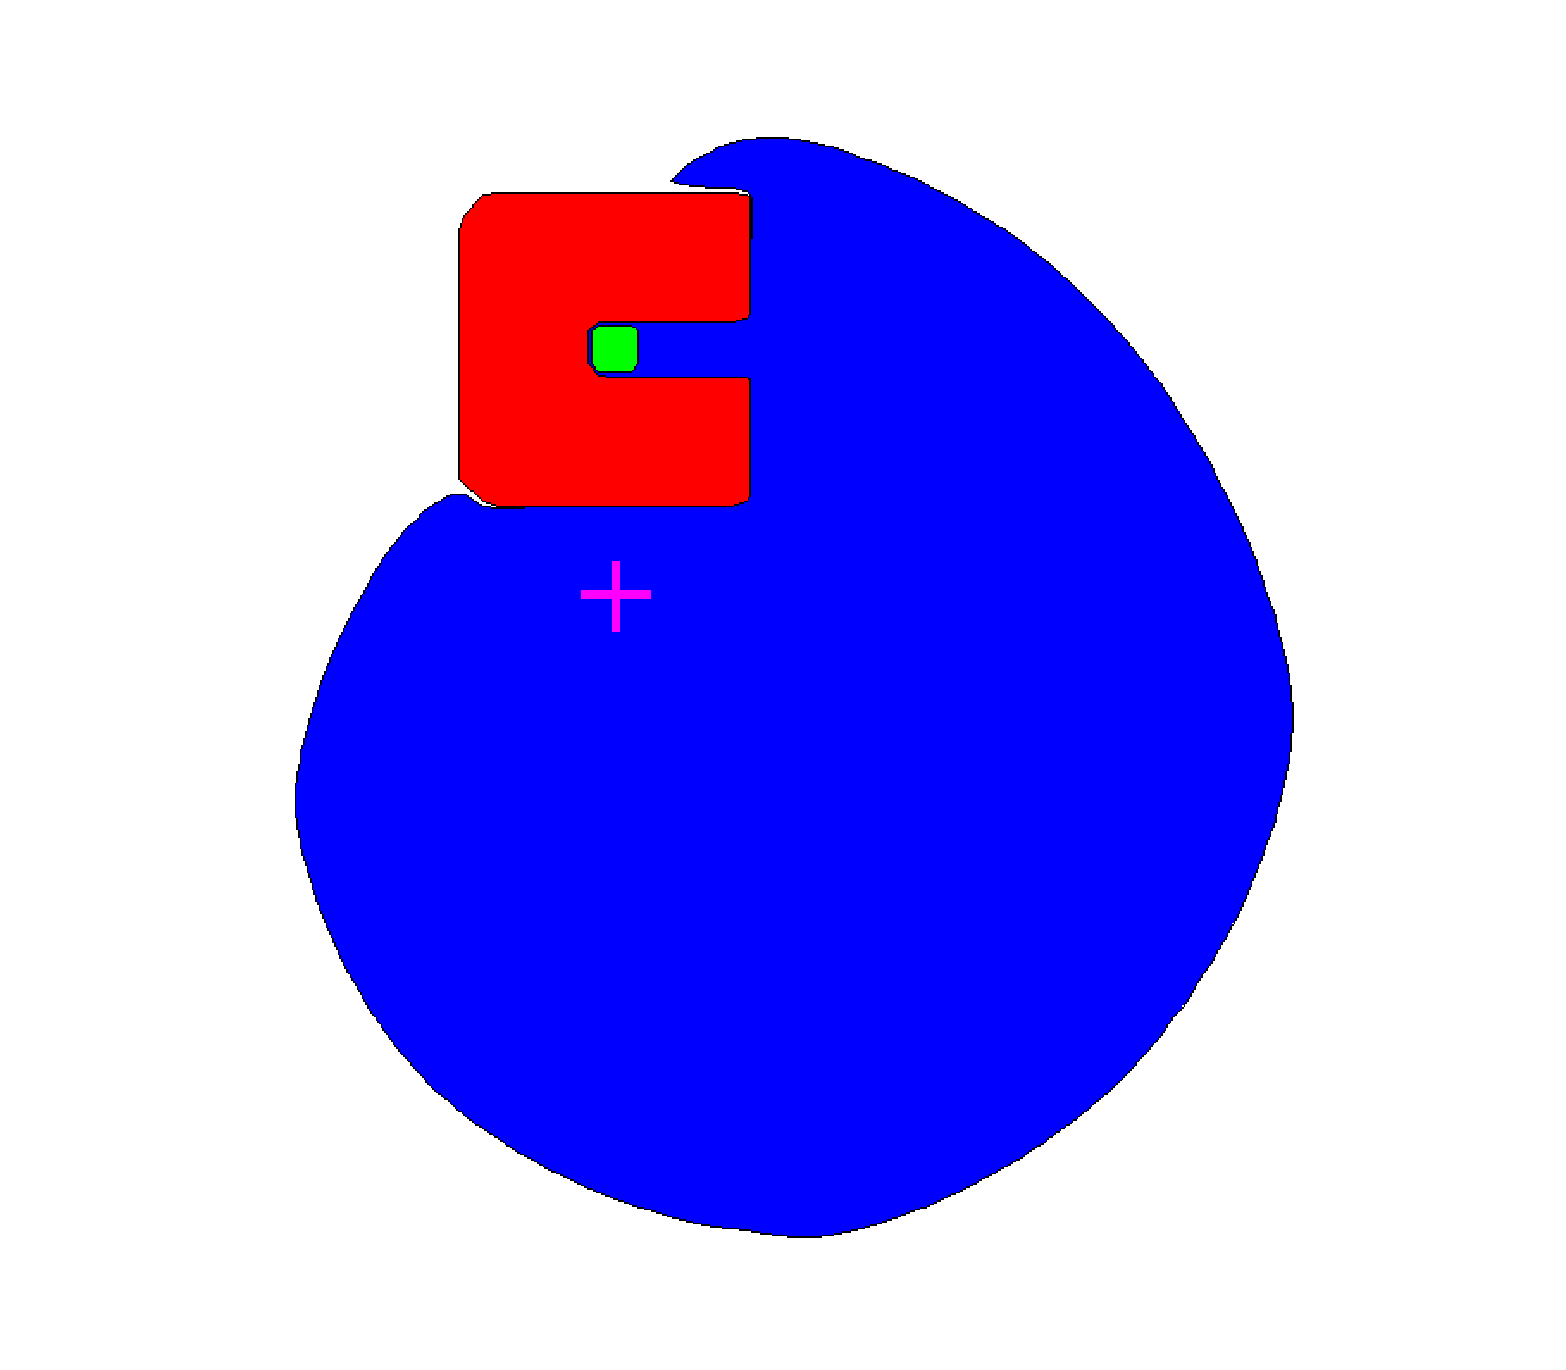
\includegraphics[scale=0.25]{figures/dynamic2Dras1.png}
    \\
    In the figure we have the 2D $RAS$ (The blue area), The obstacles (Red Area), The target set (The green area) and the initial configuration of the robot (The pink cross). From this plot we can not see the initial angular orientation of the robot since is a 2D representation, but we can better understand it from the trajectory plots below. It is important to say that the target set is not restricted only in small area of the X-axis and Y-axis , but is also limited in terms of the desired target angel $\theta$ (like in the static case). In this case we set as desired $\theta$ a small range around the angle 0 $rad$.
    \\
    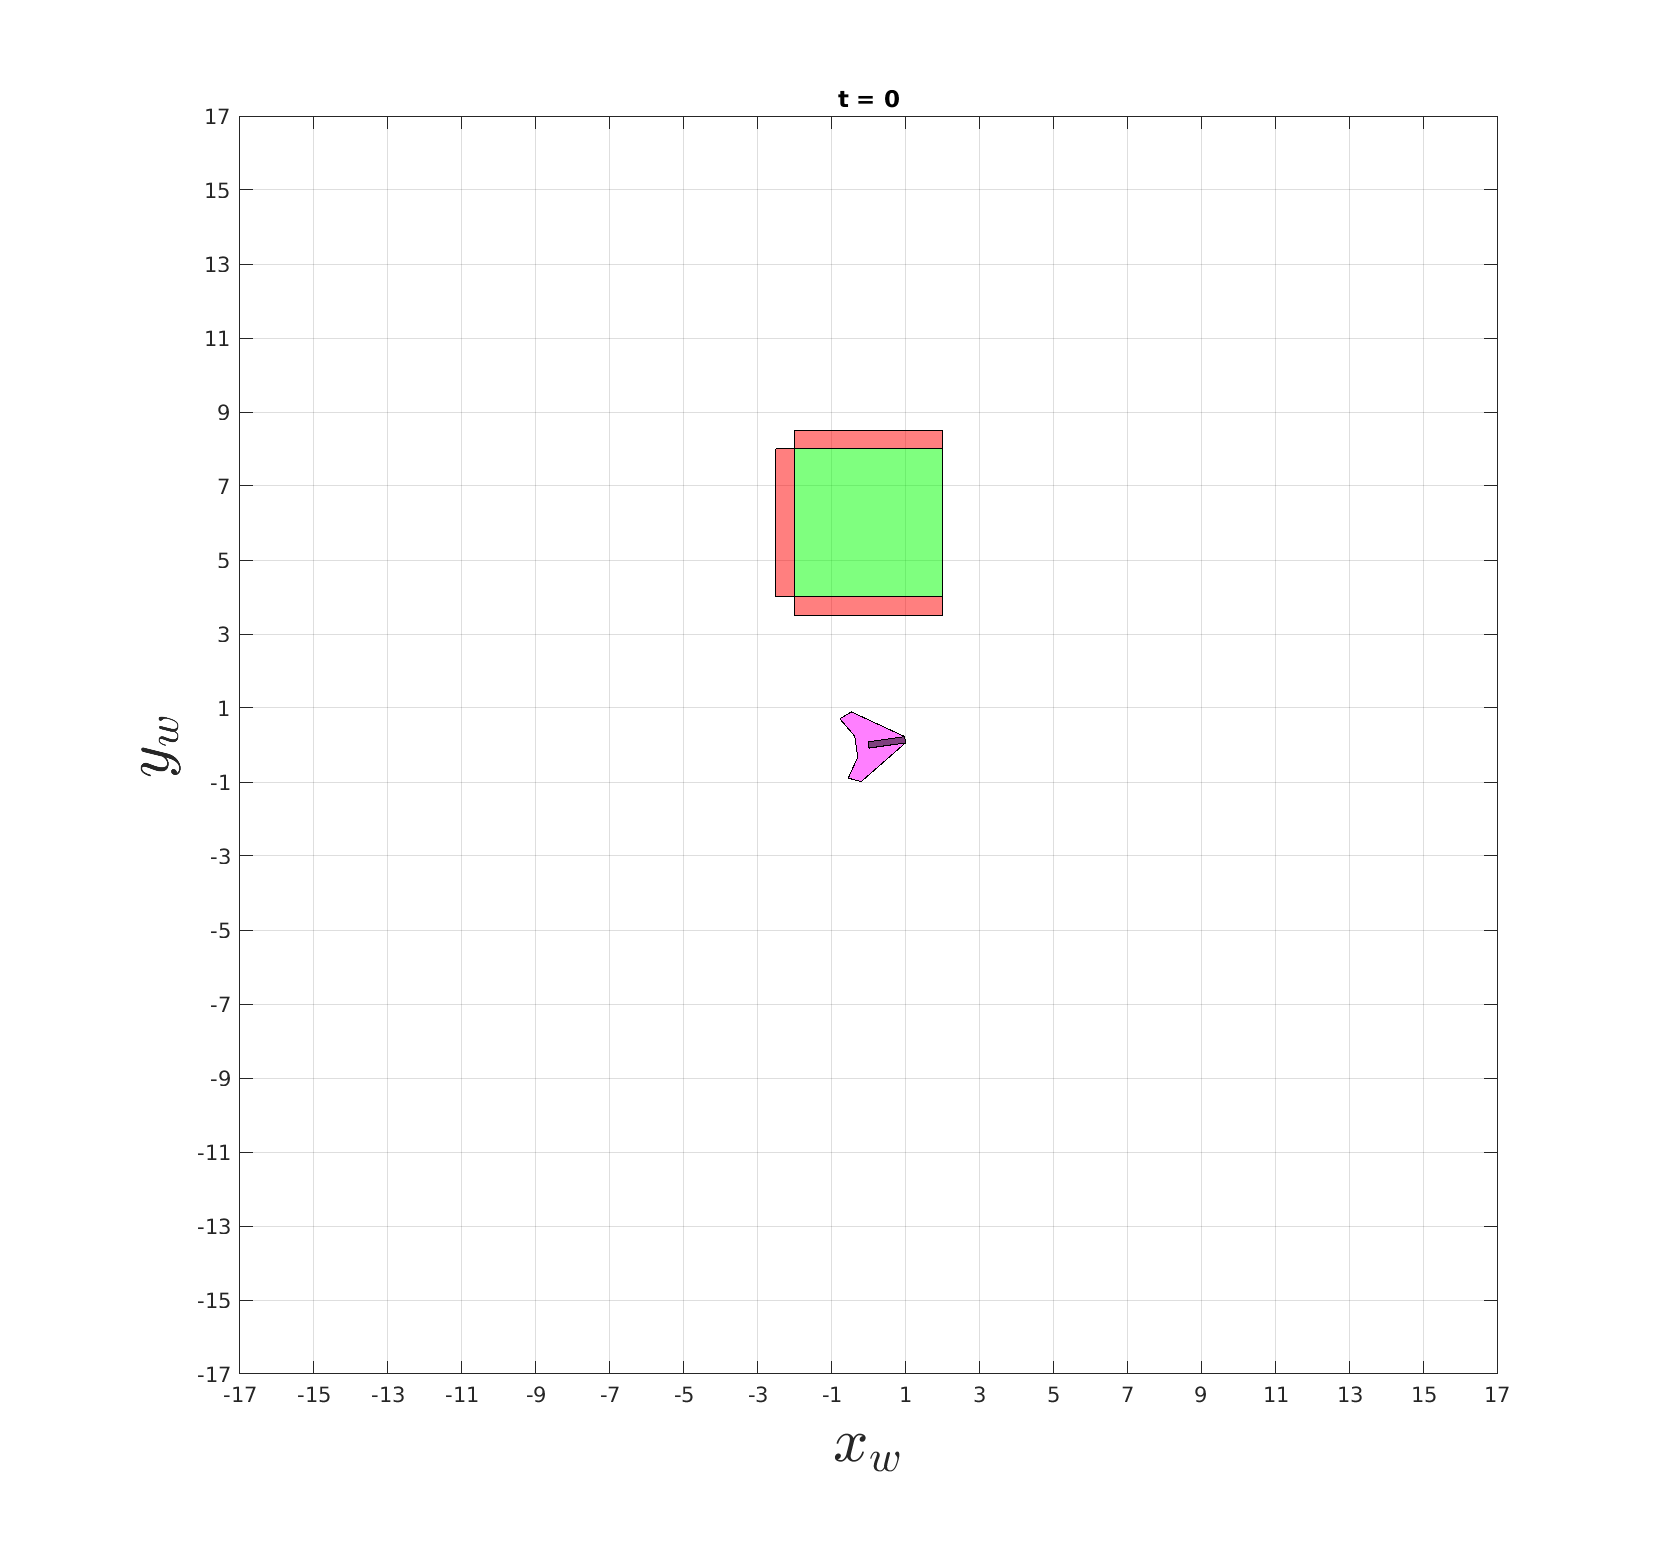
\includegraphics[scale=0.25]{figures/dynamicTRAJ1.png}
    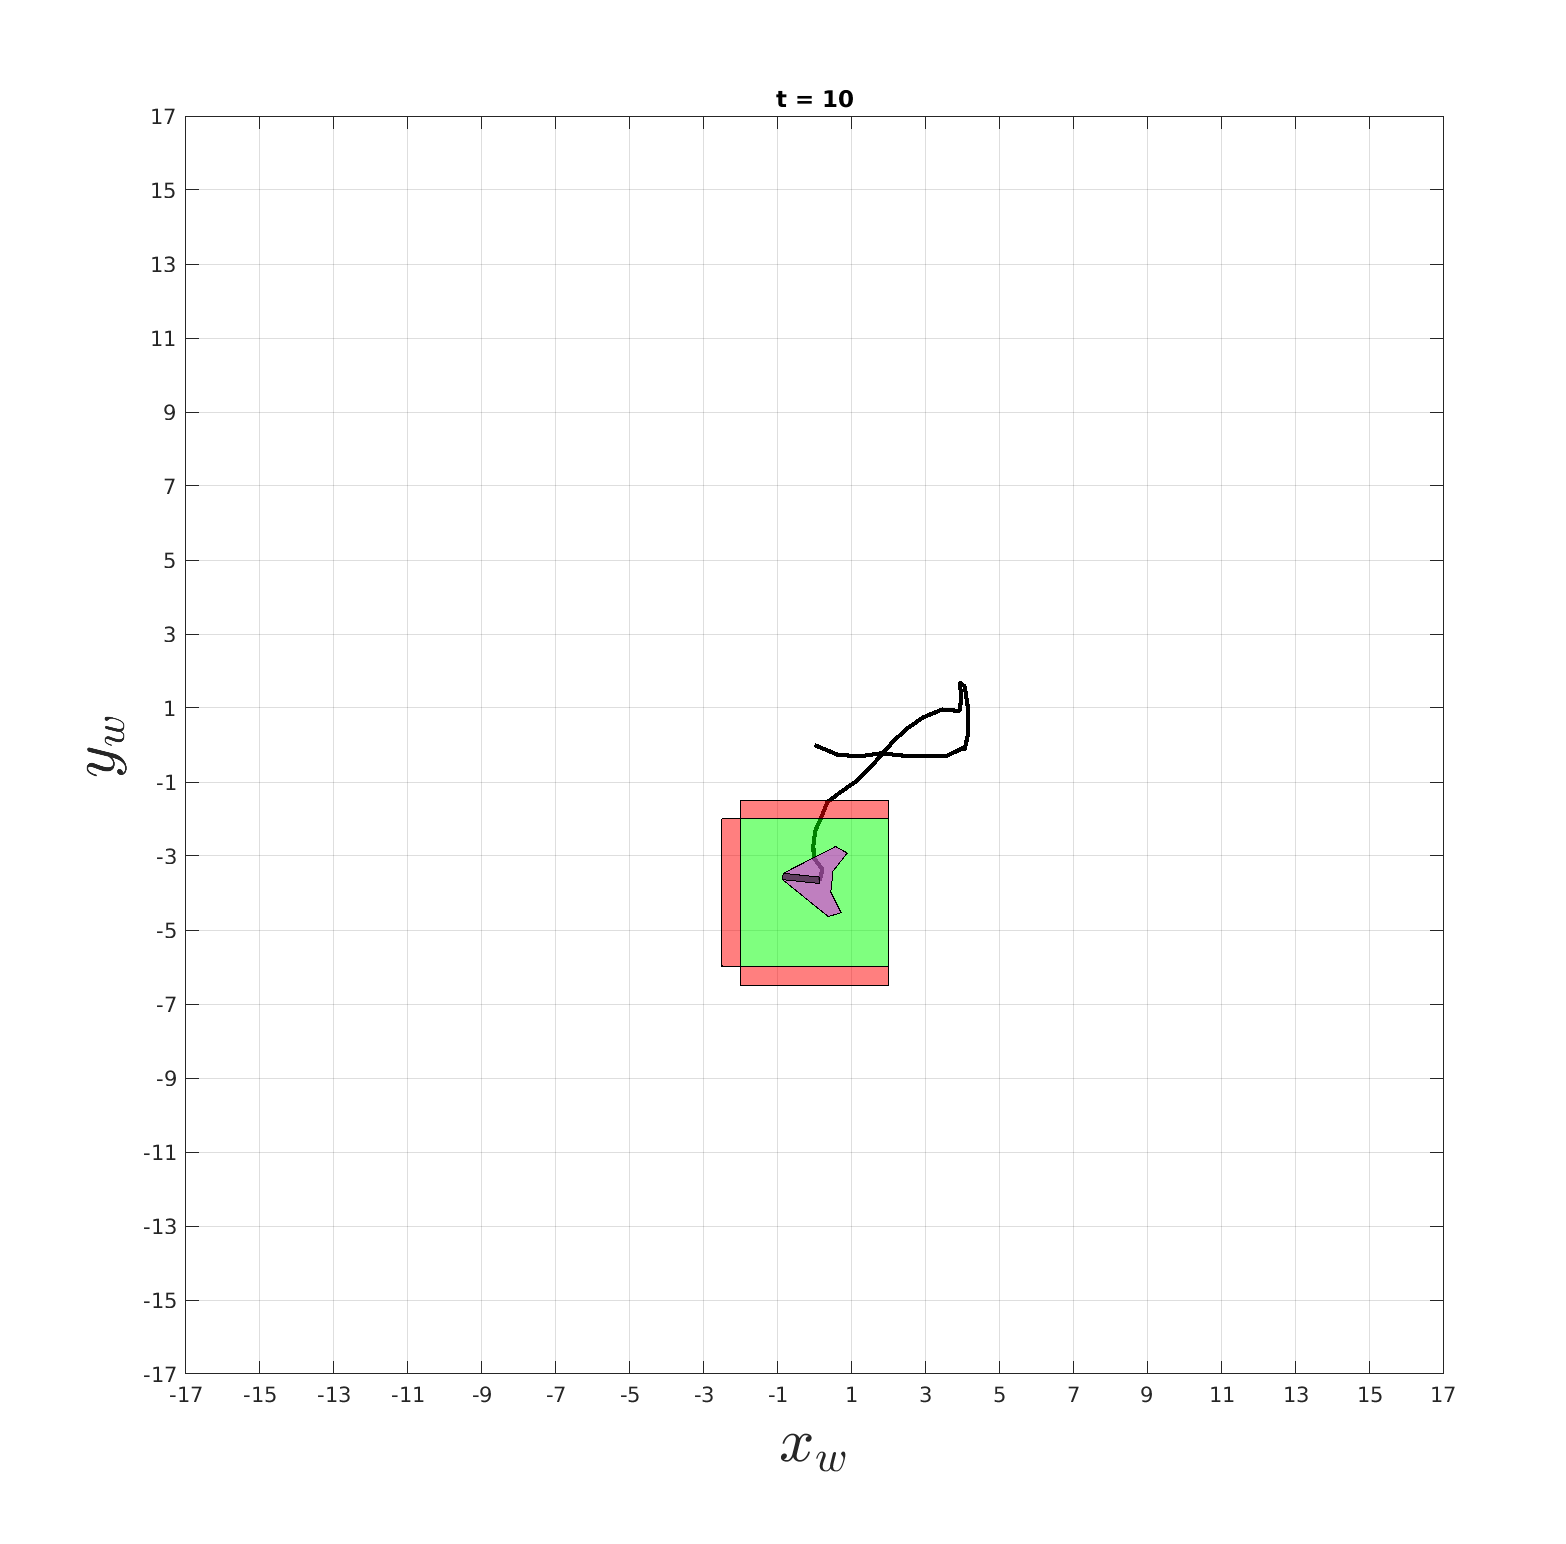
\includegraphics[scale=0.25]{figures/dynamicTRAJ2.png}
    \\
    We can see here the particular trajectory of the robot due to the movement of the target set. At time $t=10sec$ the robot is in the target set without collisions with the obstacles as expected. We can also see how it enters the target set with the desired angulation around the radiant 0
    \subsubsection{Case 2}
    The second case is similar to the previous one. In this case the only difference with the first one is the initial position of the robot. Here the robot is relatively distant from the target set, but still in the $RAS$. 
    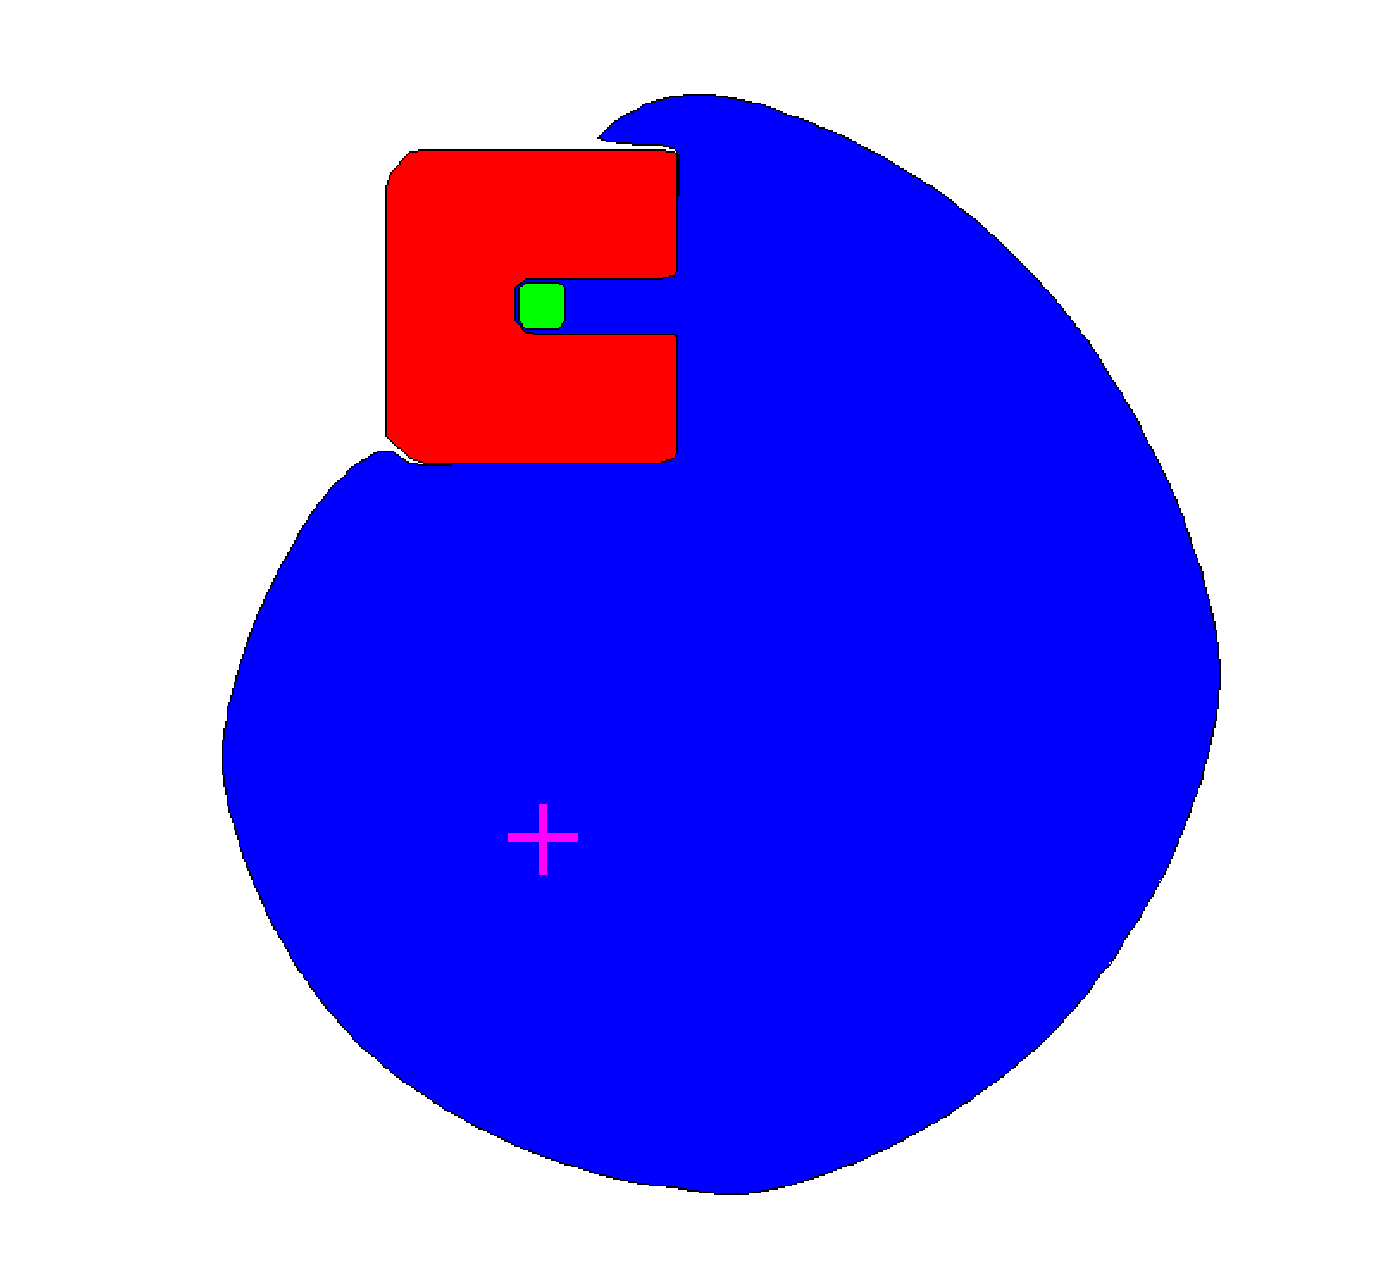
\includegraphics[scale=0.25]{figures/dynamic2Dras2.png}
    \\
    Since its initial position is still in the limits of the $RAS$ we can compute the following trajectory.
    \\
    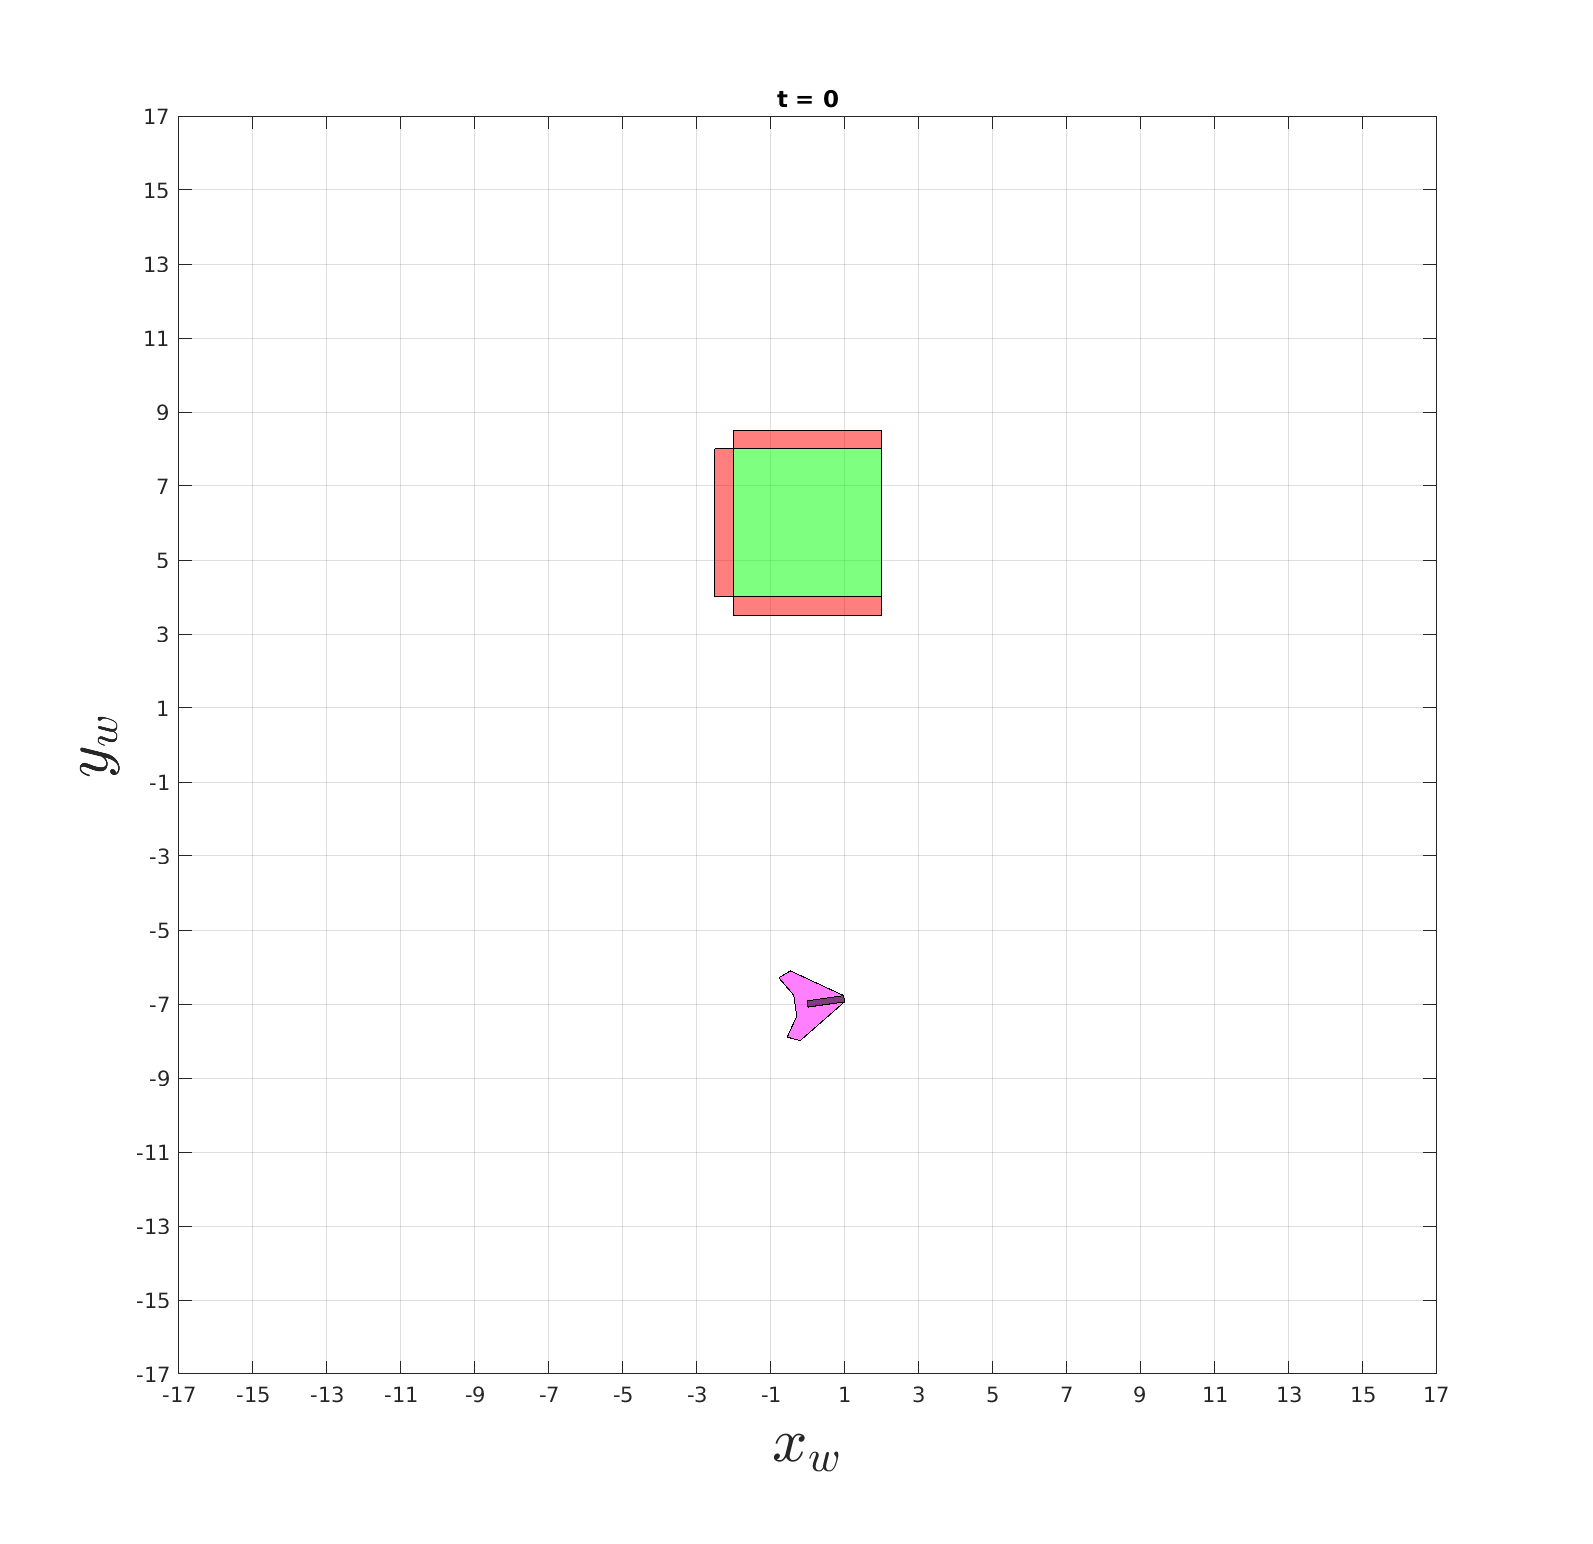
\includegraphics[scale=0.25]{figures/dynamicTRAJ3.png}
    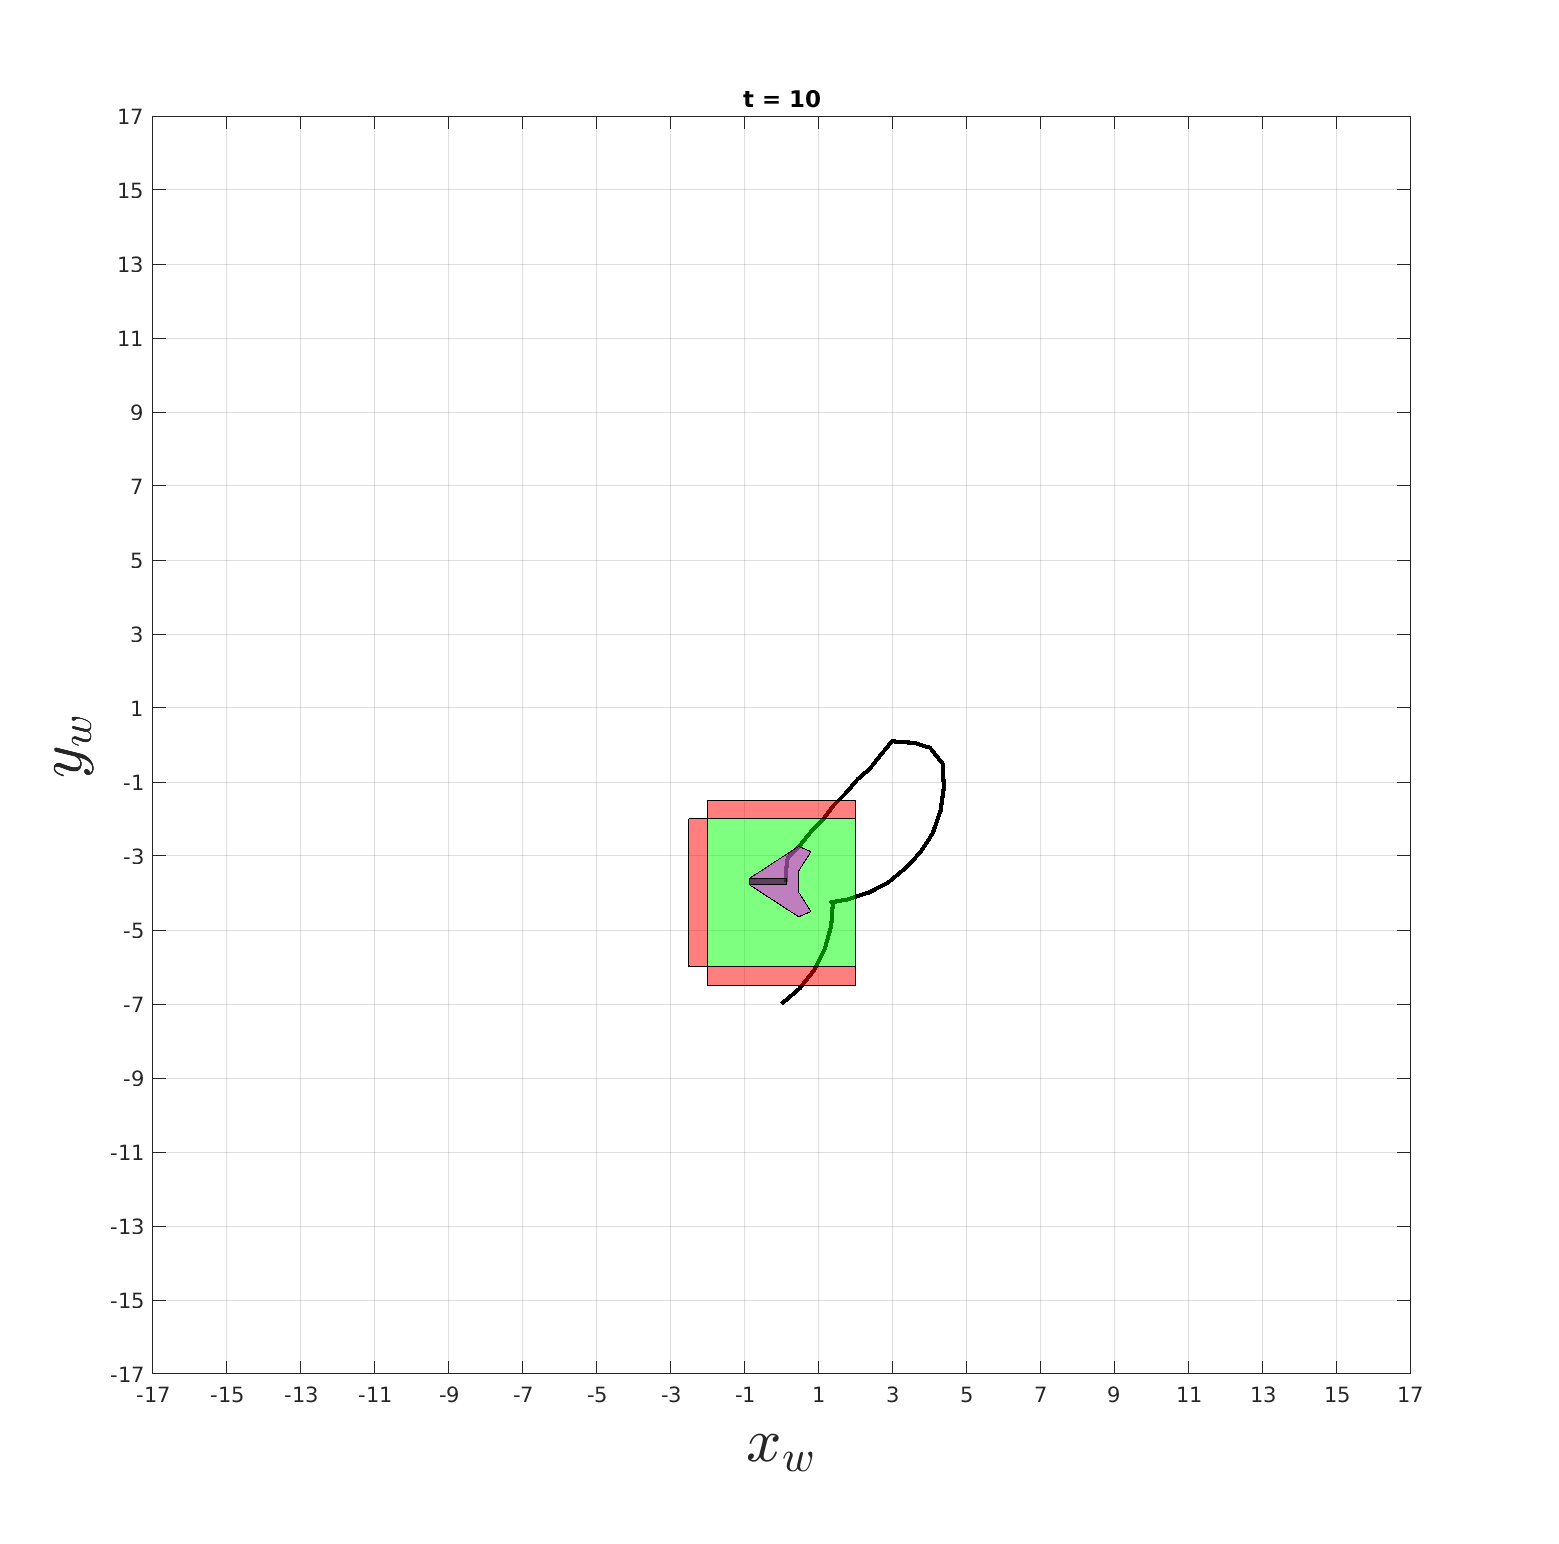
\includegraphics[scale=0.25]{figures/dynamicTRAJ4.png}
    \\
    Even in this case the Robot successfully reached the target set playing against the optimal disturbance and avoiding any obstacle.
    
    \subsubsection{Case 3}
        